\documentclass{article}
\usepackage{graphicx}
\usepackage[utf8]{inputenc}
\usepackage[T1]{fontenc}
\usepackage{subcaption}

\begin{document}

\title{Introduction and Course Overview}
\author{Felipe Glicério Gomes Marcelino}
\date{18 April 2020}
\maketitle

\section{Notes}

\subsection*{Slide 11}
\par Reinforcement learning is really important ingredient for question of how do we build intelligent machines.

\subsection*{Slide 12}
\par Some intelligent machines to imitate human behavior are difficult to build. It is because humans are not just smart
but they are good at soling problems and they are highly adaptable.

\subsection*{Slide 13}
\par Deep learning are very good at handling on unstructured because they can learn from large amounts of data and
discover patterns.

\subsection*{Slide 14}
\par Reinforcement learning provides a formalism for behavior. It is a mathematical formalization of a decision-making
problem. Reinforcement learning has a agent, an environment and the agent interacts with the environment creating a
action for a specific state of the environment. Subsequently the environment return a response taking into account the
action. 
\par Reinforcement learning has been used for things like playing games. Actually the success of the reinforcement
learning is the capacity to defeat your opponent in some games like Go(Alpha).

\subsection*{Slide 15}
\par Deep reinforcement learning removes the need to extract features manually. For example, using a CNN as policy, it
is only necessary to pre-process the image and pass this through the model. The model going to learn how to extract
the features correctly using the outcome generate by action to update the parameters.


\subsection*{Slide 21}

\begin{figure}
    \centering
    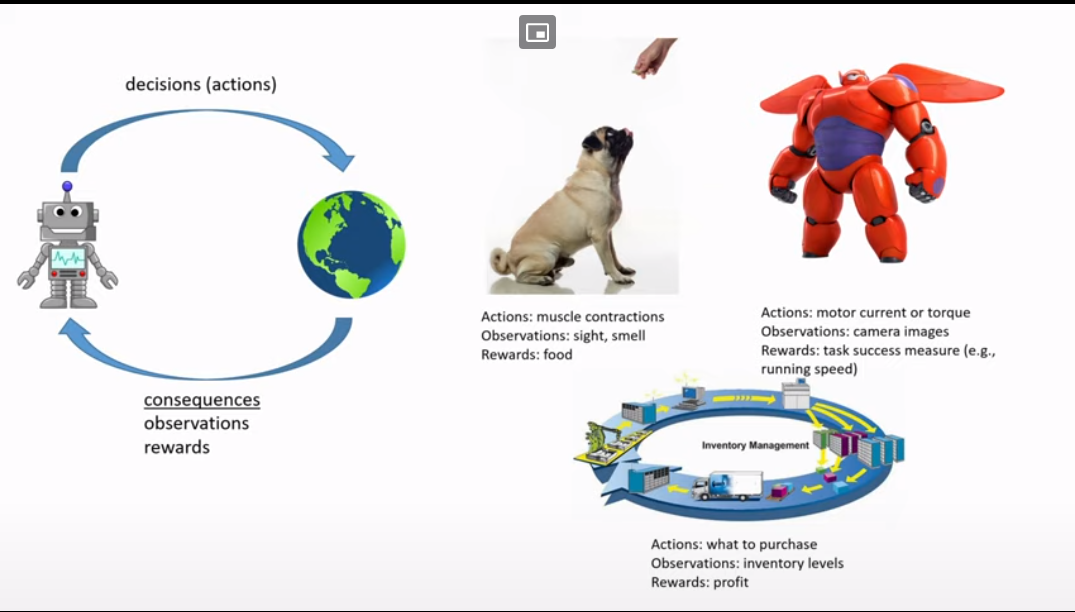
\includegraphics[scale=0.4]{cap1img/slide21.png}
    \caption{Framework of reinforcement learning}
    \label{fig:slide21}
\end{figure}

\par Figure \ref{fig:slide21} shows how the framework of reinforcement learning works. It has three elements:
\begin{itemize}
    \item Agent: Responsible to make a action using a observation space
    \item Observation Space: Data used to assist the agent
    \item Reward: Consequence of the action made by the agent
\end{itemize}

\subsection*{Slide 27}
\par Why should we study deep reinforcement learning this now?
\begin{enumerate}
    \item  Advances in deep learning - We can create complex architecture networks and training them using
        sophisticates techniques to understand  high dimensional observation spaces, such as images.
    \item  Advances in reinforcement learning - We have algorithms with favorable numerical properties, they are
        stable to use and reliable. It can converge to good solutions.
    \item Advances in computational capability - More power to process, more advanced tasks can be achieved
\end{enumerate}

\subsection*{Slide 31}%
\label{sub:Slide 31}

\par 
\begin{enumerate}
    \item Basic reinforcement learning deals with maximizing rewards
    \item This is not the only problem taht matters for sequential decision
    \item Inverse reinforcement learning - Learning reward functions from example
    \item Transferring knowledge between domains (transfer learning, meta learning)
    \item Learning to predict and using prediction to act
\end{enumerate}

\subsection*{Slide 42}%
\label{sub:Slide 42}
\par How do we build intelligent machines? It is possible to program and execute in a computer a imitation of the
brain. It is possible to emulates the behavior of the brain. However, each of these parts from brain are themselves
quinte complicated to emulate. 

\par So the idea behind reinforcement learning is implement learning algorithms that can acquire the functionality of
those parts from brain. 

\subsection*{Slide 46}%
\label{sub:Slide 46}
\par Algorithms used by deep reinforcement learning field must be capable to interpret rich sensory inputs, as images
and choose a complex actions. Consequently, it is necessary to use deep learning as base algorithms. Deep = can
process complex sensory input, and anslo compute really complex functions. 



\end{document}
